\documentclass[12pt]{article}
\usepackage{graphicx}
\usepackage{amsmath}
\usepackage{amssymb}
\usepackage[authoryear]{natbib}
\usepackage{enumerate}
\usepackage{booktabs}
\usepackage{siunitx}
\newcolumntype{d}{S[ input-open-uncertainty=, input-close-uncertainty=,
      parse-numbers = false, table-align-text-pre=false,
      table-align-text-post=false ]}
\usepackage{pdflscape}
\usepackage{hyperref}

\hypersetup{ colorlinks, citecolor=black, filecolor=black, linkcolor=black,
    urlcolor=black }
\setlength{\parindent}{0pt}
\usepackage[parfill]{parskip}
\date{July 2023}
\title{Retirement Consumption: Evidence from UK Pension Reform}
\author{INSERT NUMBER HERE}
\usepackage[letterpaper, margin=1.1in]{geometry}
\linespread{1.25}

\begin{document}

\newpage
\maketitle
\tableofcontents
\newpage

Classical economic theory suggests that retirement annuities, which provide a
guaranteed income stream until the end of life, should be highly valued by
individuals as a way to insure against late death \cite{yaari_65}. However, in
developed countries, rates of annuitisation are far below the levels that theory
predicts - this phenomenon has been termed the "annuity puzzle". The literature
has suggested several reasons for this, but there is no consensus about which
mechanism is dominant. I exploit early retirees' consumption responses to a
reform to annuity policy in the UK to add to this literature. [\textbf{Add
            something once I have a conclusion}].

In the UK, adults have three methods of funding retirement: the state pension;
defined benefit (DB) employee pension schemes, which provide an income in
retirement based on years of service and a function of wages; and defined
contribution (DC) pensions, under which individuals save and invest in a
tax-advantaged account that is usually supplemented with employer contributions.
Under the 2010-2015 coalition government in the UK, the law regarding the use of
private DC pensions at retirement changed. Individuals were no longer forced to
annuitise their pension pots and could access them in a variety of ways, such as
a lump sum withdrawal or income drawdown, involving a steady withdrawal of
assets from the pension pot -- common advice is to take 4\% a year. Subsequently
the number of annuities sold in the UK dropped precipitously.

In this paper, I first use the policy reform as a discontinuity to measure the
impact of forced annuitisation on the consumption levels of individuals in the
first few years of retirement. Given that the reform was implemented suddenly
and without advanced notice before the Spring 2014 budget, I claim that
individuals who retired in 2015, 2016 or 2017 are otherwise similar to those who
retired in 2011, 2012 and 2013 except for the fact the later retirees do not
need to annuitise their DC pension pots. Therefore, I can use a regression
discontinuity to identify the effect that forced annuitisation has on the
consumption of retirees.

I then test two competing hypotheses for the annuity puzzle: bequests and
pessimistic life expectancy. The annuity puzzle was first identified by
\cite{yaari_65} and is a classed as a problem since standard economic theory
cannot explain the lack of annuitisation that is observed in the real world. Two
possible explanations are bequests and life expectancy: individuals want to
leave an estate for their heirs to inherit and they cannot do this if they
annuitise their wealth; or individuals may believe they will not live as long as
annuity providers think they will and therefore annuities that are on the market
do not appear to be good value. Depending on the reason for the lack of
annuitisation in the UK, the consumption response of retirees to the pension
reform will differ. If individuals do not annuitise because of pessimistic life
expectancy their consumption should increase after the reform. If, on the other
hand, individuals do not annuitise \ because of a bequest motive, consumption
should not change much as a result of the reform.

I will solve lifecycle models (\textbf{maybe add something about lifecycle
    models here}) for both of these cases and simulate consumption decisions with
and without forced annuitisation. I will then use a variety of empirical models
to measure the consumption change in early retirement that resulted from the
policy reform. The sign and magnitude of this change will be indicative of the
mechanism causing the annuitisation problem.


The importance of retirement policy to individuals in the UK is growing. The
number of individuals of pensionable age is expected to increase from 11.9
million in 2020 to 15.2 million in 2045 according to the latest projections from
the Office for National Statistics (ONS) and for every 1000 people of working
age there will be 341 of pensionable age in 2045 compared to 280 in 2020
\cite{ons_population_predictions_2020}. The increase in absolute and relative
numbers of elderly people makes retirement policy more consequential. Moreover,
private DC pensions are becoming increasingly common and are predicted to grow
as current cohorts age \cite{cribb_karjalainen_ifs_2023}. Therefore, policies
regarding how private pensions can be accessed will have a larger impact on
overall welfare for retirees.

Moreover, understanding how retirees spend their money over retirement is an
important policy question of its own. If retirees spend too much in early
retirement, the state may need to provide for them towards the end of their
lives. This has implications for government budgets, especially since population
aging means more individuals will require expensive end of life care. On the
other hand, if retirees over-save and do not spend, the economy may be
dynamically inefficient whereby the capital stock is too high because
individuals save too much for retirement and for bequests. In this case
consumption per capita could be increased if savings were decreased.


\subsection{Literature review}
My paper builds on three main strands of literature: that of the annuity puzzle,
exploring reasons that some retirees choose not to annuitise; the retirement
saving puzzle, which seeks to explain why retirees drawdown assets slowly, ; and
lifecycle models, whereby the above problems are explained using a tractable
model of human decision making.

\cite{yaari_65} showed that under standard assumptions we would expect
individuals to annuitise all of their wealth at retirement to insure against the
risk of long life. Since then there has been much literature discussing possible
reasons that people do not annuitise. \cite{finkelstein_porteba_2002} and
\cite{finkelstein_porteba_2004} find evidence of adverse selection, thereby
making the 'money's worth' of annuities lower for the general population as
opposed to the population of annuitants. However, they also find that theory
would still predict annuitisation.

\cite{friedman_warshawsky_qje_1990} show that annuitisation decisions can be
fully explained by a mixture of bequest motives and actuarily unfair annuities.
They solve an augmented life-cycle model with a range of parameters on how
severe the rate of return is on the annuity versus market rates. For plausible
values they find that individuals would optimally not annuitise much wealth.
Similarly to \cite{finkelstein_porteba_2004},
\cite{friedman_warshawsky_chicago_1988} show that there is a significant
difference between the life expectancy of annuitants and the general population
in the American annuity market but this cannot fully explain the annuitisation
puzzle. Only when bequest motives are added to the model can annuitisation rates
be rationalized.

\cite{lockwood_red_2012} builds on this and shows that a realistic bequest
motive in lifecycle simulations achieves realistic annuitisation rates. He
solves a simple lifecycle model with bequest motives taken from several recent
papers in the literature. The bequest motives he picks therefore match other
important aspects of the lifecycle model such as how much individuals actually
bequest and how rich individuals are when they bequest.

\cite{lockwood_aer_2018}

\cite{vidalmelia_lejarragagarcia_munich_2004} have some interesting results.
Need to talk about that.

\textbf{There are some more papers I will include here.}

\section{Data and Policy reform}

\subsection{Data}

The main dataset I use is the English Longitudinal Study of Ageing (ELSA)
\cite{main_elsa_citation}. ELSA picks individuals over the age of 50 to survey
every two years until death. If individuals leave the survey, ELSA replaces them
so that it is representative of the over 50 population in the UK. Individuals
are asked a range of questions relating to their income and wealth as well as
expectations about the future. One benefit of using ELSA is that it includes
data on pension types for individuals who are working. Therefore, I can
differentiate between individuals who have a DC pension and those who have a DB
pension. There have been 9 waves of ELSA data collection -- the first was in
2001 and collections happened every two years thereafter.

Importantly, ELSA also includes information on pension size calculated by the
Institute for Fiscal Studies (IFS). This is only available up to and including
wave 5 (which was collected in 2010 and 2011) at which point I use a real return
of 3\% to predict forward the pension wealth variable until retirement. ELSA
also includes a measure of all non-housing financial wealth which I use in some
specifications because of these issues with pension wealth data. Due to slight
differences in the ELSA questions between years, I use `Harmonized ELSA'
\footnote{This analysis uses data or information from the Harmonized ELSA
    dataset and Codebook, Version G.2 as of July 2021 developed by the Gateway to
    Global Aging Data. The development of the Harmonized ELSA was funded by the
    National Institute on Aging (R01 AG030153, RC2 AG036619, R03 AG043052). For more
    information, please refer to https://g2aging.org/.} which ensures that variables
are comparable across waves. Since this only includes a subset of the questions
in ELSA, I supplement it with variables taken directly from the data such as
questions that deal with life expectancy.

ELSA also includes questions on expenditures. In particular, individuals are
asked how much they consume across a range of broad categories including
in-house food consumption, out-of-house food consumption, leisure consumption,
clothes consumption and consumption on utility bills and rent.

I also use `life tables' from the UK's ONS. These provide me with the risk of
death for each age group. Since the tables are produced until age 120, I adjust
them to make death certain at age 110 as is common in the literature
\cite{odea_sturrock_rest_2023}. I transform these so that I have risk of death
conditional on being a given age since this is what I use in the life cycle
simulations. I also use these objective probabilities to calculate annuity
prices for individuals.

To illustrate the effect that the reform had on sales of annuities in the UK I
obtained product data from the Financial Conduct Authority. These track the
sales of different financial products overtime including data on annuities.

Life expectancy impacts the decision to annuitise for two reasons. Firstly, it
directly impacts the price that an annuity will cost for individuals. Older
individuals and those with pre-existing health conditions generally can buy an
annuity that provides a greater income stream than individuals who are younger.
Secondly, private information about life expectancy impacts the perceived value
of an annuity. If an individual expects to outlive the general population, an
annuity, at a given price, will appear a much better deal to them. Likewise, an
individual's life expectancy will change their decision on how to consume and
save through retirement.

To calculate subjective life expectancies from ELSA data, I follow
\cite{odea_sturrock_rest_2023}. Individuals were asked “What are the chances
that you will live to be age X or more?” where X changed depending on the age of
the interviewee. If individuals were under 65 then X was 75, if individuals were
66 and older they were asked the age that was 11 to 15 years older than them and
a multiple of 5. From wave 3 respondents were also asked “What are the chances
that you will live to be age 85 or more?” if they were under 70. As most recent
retirees are under 70 we therefore have two data points. I first drop from the
data individuals who think it is more likely that they reach a higher age than a
younger age since this shows a misunderstanding of the question. I then add as a
third data point their objective chance of reaching 110 according to the ONS
life tables. I fit these three points to a Weibull distribution, which is
commonly used by demographers to estimate how populations will age, using
non-linear least squares. Then I create subjective survival tables using
parameters from the Weibull distribution.

\textbf{I could go into more detail here? Maybe I should. Add equation etc}


\subsection{Policy reform}

Successive governments in the UK have attempted to reform both the public and
private pension system. Prior to 1987, participation in private schemes was
limited to employees of firms that had offered them, and there were few
alternatives to the public state pension or DB scheme that a public sector
employer would offer. From 1989, individuals in the UK were allowed to open tax
advantaged self-invested personal pensions alongside any pension their employer
offered. The 2004 Finance Act rationalised taxation rates on DB and DC pensions.
The rules for DC pension pots were such that individuals had to buy an annuity
after optionally taking a maximum of 25\% of the pot as a tax free lump sum
withdrawal. DC pension pots were accessible from age 55 and most required that
they be accessed before the age of 75.


In the June 2010 budget, the coalition government made the first of two key
reforms it would make to the pension system between 2010 and 2015. The 2010
policy reform created a minimum income requirement above which individuals would
not need to annuitise more \cite{finance_act_hmt_2011}, this meant high income
retirees would not need to annuitise their wealth. The income requirement was
set at £20,000. This meant, for example, that an individual who was a member of
a DB scheme paying them £20,000 a year would not need to annuitise their DC
pension pot. However, the relatively high minimum income requirement meant that
most individuals still had to purchase an annuity.

In spring 2014, George Osbourne announced the so called `pensions freedom act'
scrapping the minimum income requirement and eliminating the compulsory
annuities market \cite{pen_freedoms_hmt_2014}. One government minister
infamously brought the message home by saying pension pots `can be used to buy
Lamborghinis' if retirees wanted to \cite{guardian_lambos}. The government also
announced plans to make switches between DB and DC pension schemes possible
although this was only realised in the next parliament -- future research could
explore the impact of this second reform on the consumption and saving decisions
of retirees.

The impact of the reforms on annuity demand has been documented by
\cite{cannon_et_al_nier_2016}. Using data from the Association of British
Insurers, they show that annuity demand dropped by 75\% from its maximum in
2011. Figure \ref{fig:annovertime} shows purchases of annuities overtime and
demonstrates the sharp decrease in purchases that happened from 2014 to 2015.
There was an increase in the number of pensions that were being accessed using
an income drawdown product, but these only partly account for the drop in
annuitisation as is shown by the graph.
\begin{figure}[h]
    \caption{New pension pots accessed }
    \centering
    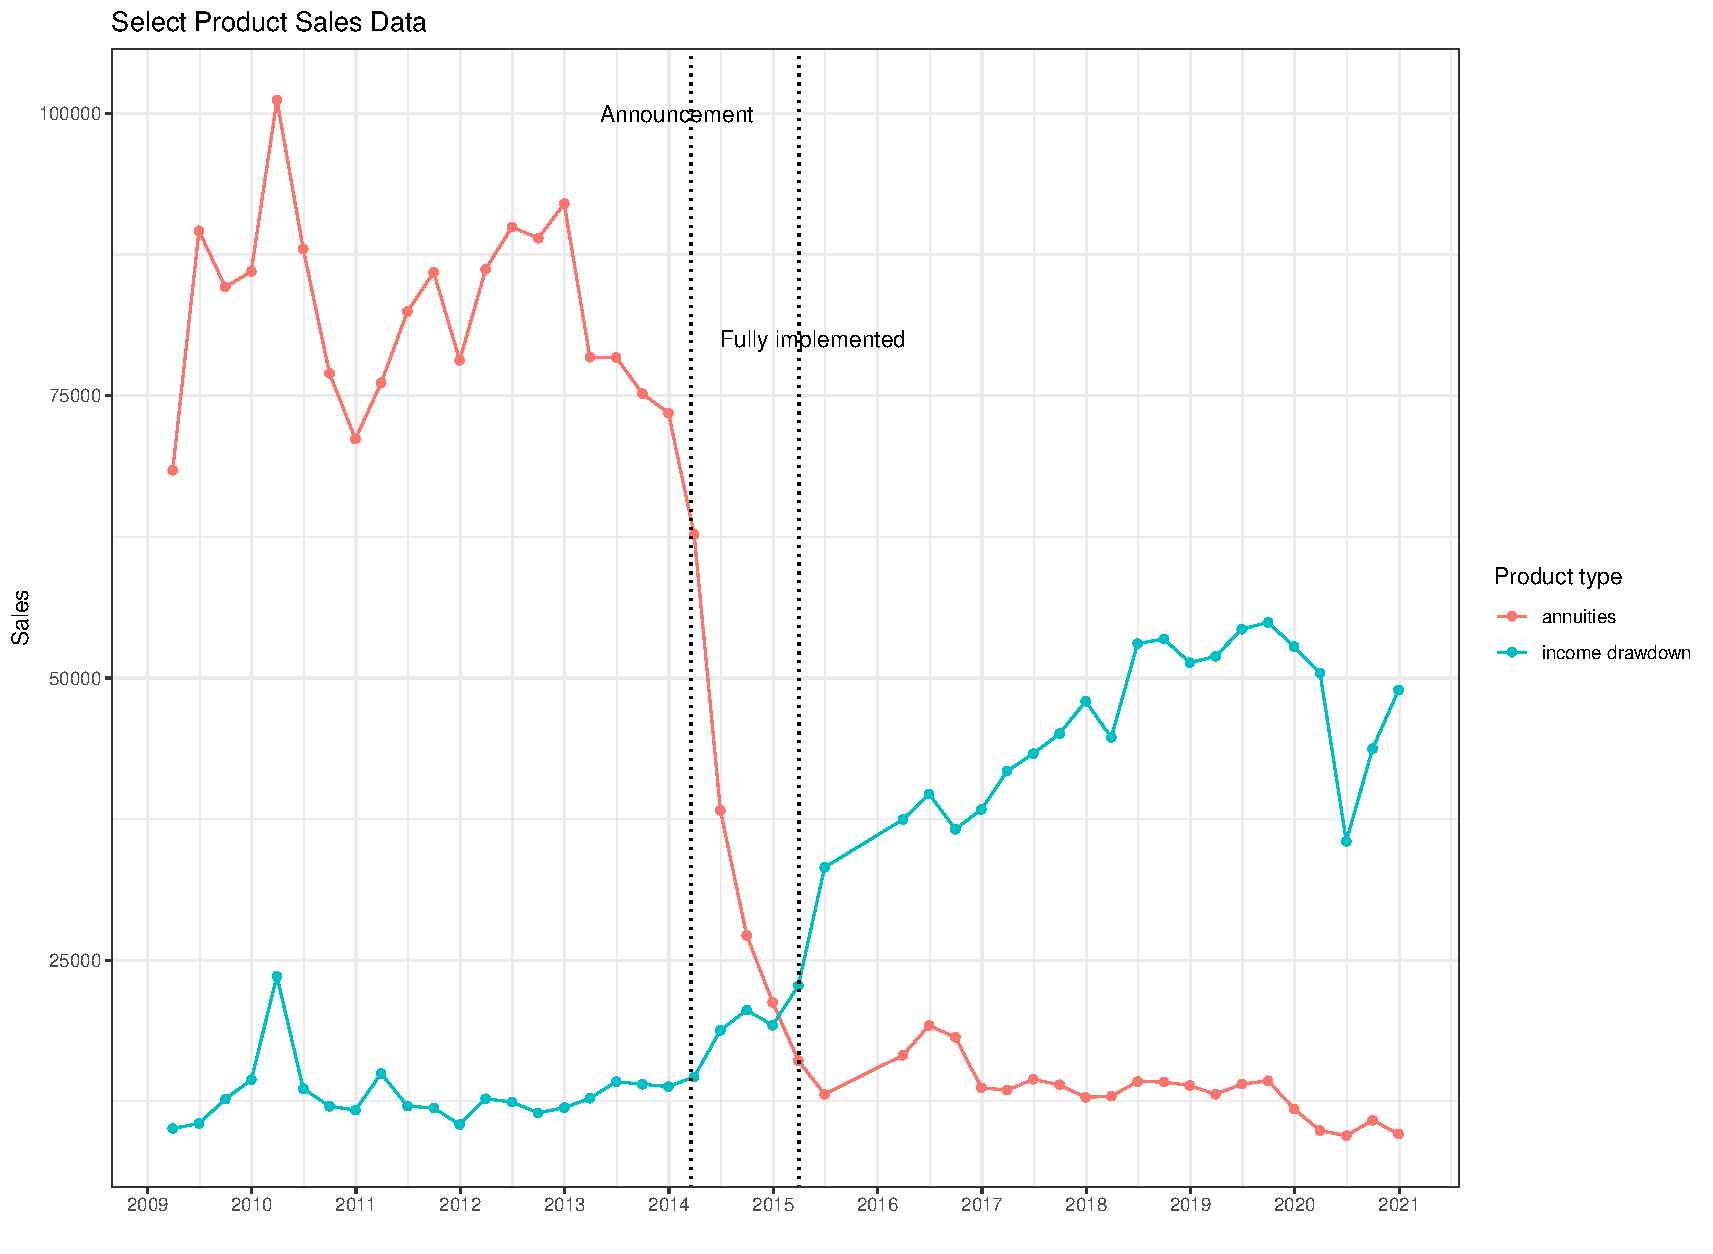
\includegraphics[width=0.7\columnwidth]{figures/annuity_overtime.pdf}
    \label{fig:annovertime}
\end{figure}

\begin{figure}[h]
    \caption[Caption for LOF]{How pension pots are accessed\protect\footnotemark}
    \centering
    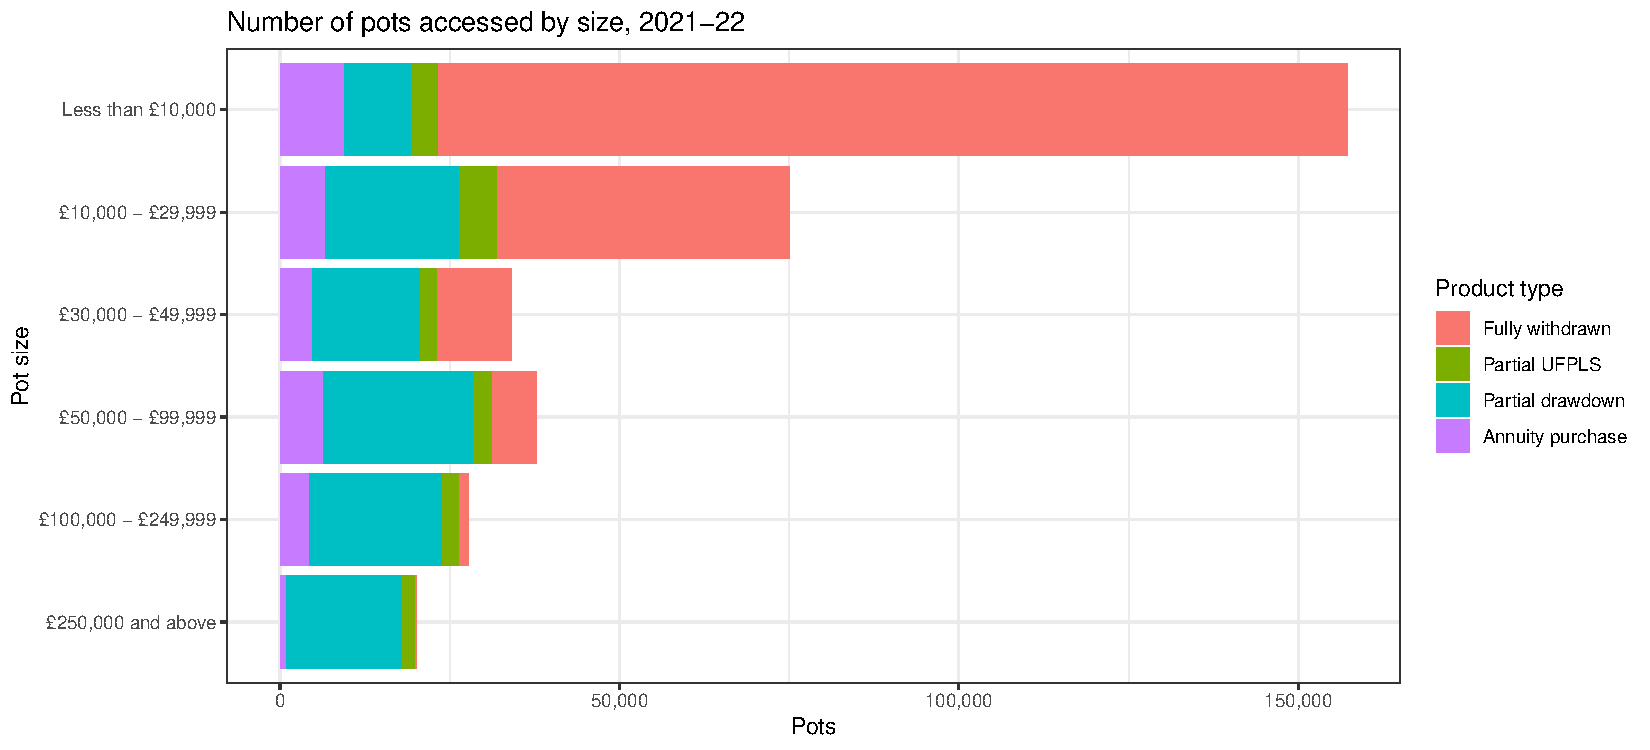
\includegraphics[width=0.7\columnwidth]{figures/annuity_pot_sizes.pdf}
    \label{fig:ann2122}
    \
\end{figure}
Figure \ref{fig:ann2122} shows the distribution methods to access pension pots
at retirement in 2021-22. In 2021, 196,736 pots were fully withdrawn at
retirement, accounting for over 50\% of pots. Prior to the policy reform this
was not the case -- most defined contribution pensions were accessed through
annuities.


Also of specific interest to the annuity market was the European Union's `Equal
Treatment in Goods and Services Directive' of 2004. This prohibited
discrimination in the provision and cost of goods and services based on sex. Up
until 2011, there was a clause that stated insurers were allowed to charge
different premiums if it was based on evidence that sex is correlated with
different amounts of risk. However, in March 2011, the European Court of Justice
ruled that insurers were not allowed to charge different amounts and gave them
until December 2012 to implement the ruling. This change meant that annuity
products could no longer be priced differently for men and women in the UK.
However, given that this change was implemented two years before the pension
freedoms act it will not impact my results.

\footnotetext{Partial UFPLS (uncrystallised funds pension lump sum) is similar
    to Partial drawdown but with a different tax schedule. With partial drawdown
    you take the whole 25\% tax free amount at once whereas with UFPLS you only
    claim the tax relief on 25\% of the amount you are taking out. This option
    is better if you may want to buy another retirement product in the future
    such as an annuity. }


\subsection{Covariate Balance}

Table \ref{tab:sum_stats} shows various summary statistics for each variable of
interest from ELSA and the ONS.

As required, retirement year is between 2011 and 2013 for the control group and
2015 and 2017 for the treatment group. However, as discussed above their ELSA
interview date is after or the same as the retirement year because we are
tracking consumption in retirement.

The second retirement group, those who retired post-reform, is small with just
728 non missing observations for gender as opposed to 941 individuals in the
control group. The control group are more female, retired at a slightly younger
age and expected to retire slightly earlier. This could be because this period
was affected by the increase in the state pension age for women from age 60 in
2010 to age 65 in 2018. Since this change happened gradually and ocurred over
the whole period I do not expect it to influence the results. The DifferenceAge
row tracks the difference between expected and actual retirement age.

The treatment group has higher financial wealth with a median of £66,000 at the
time of interview as opposed to £55,000 in the control group. Likewise, the
second group are more likely to have held a DC pension at some point and have
much more money in them. Both groups are equally likely to have a DB pension
with roughly 44\% of individuals across both samples having a DB pension. In
general, DB pensions are more prevalent than DC pensions in the data, this
reflects the same trend that is observed in the general UK population. Home
ownership is roughly equal across groups although the second group have slightly
higher housing wealth.

Both groups are similarly long-lived when using ONS life tables to calculate
life expectancy based on gender, age and the year the interview was carried out
in. Subjective life expectancies are also similar across groups, with
individuals expecting to live another 21 years as opposed to the 24 that the ONS
would expect them to live.

Unfortunately, some consumption data is missing for some individuals. The food
categories have the least missing data and the leisure consumption category has
the most missing data.


\textbf{Maybe add in prob of survival to age 85 or 90 or something}
\textbf{Also add in an indicator for living alone or living with someone else}

Overall, the groups appear to have slightly different wealth profiles with the
treatment group being richer and slightly more likely to have DC pension wealth.
On key demographic characteristics, however, the groups are similar. The
difference in retirement age between the two groups can be mostly explained by
the difference in expected retirement age meaning that individuals have not en
masse decided to delay retirement and avoid annuitisation. Moreover, for the
regression discontinuity models I only use individuals who have a DC pension so
it does not matter that there are more individuals with DC pensions in the
second group.
\begin{landscape}
    \tiny
    \begin{table}

\caption{Summary statistics \label{tab:sum_stats} }
\centering
\fontsize{10}{12}\selectfont
\begin{tabular}[t]{lrrrrrrrrrr}
\toprule
\multicolumn{1}{c}{ } & \multicolumn{2}{c}{Max} & \multicolumn{2}{c}{Mean} & \multicolumn{2}{c}{Median} & \multicolumn{2}{c}{Min} & \multicolumn{2}{c}{Non Missing} \\
\cmidrule(l{3pt}r{3pt}){2-3} \cmidrule(l{3pt}r{3pt}){4-5} \cmidrule(l{3pt}r{3pt}){6-7} \cmidrule(l{3pt}r{3pt}){8-9} \cmidrule(l{3pt}r{3pt}){10-11}
 & Control & Treat & Control & Treat & Control & Treat & Control & Treat & Control & Treat\\
\midrule
Gender & 1.0 & 1.0 & 0.470 & 0.495 & 0.0 & 0.0 & 0.0 & 0.0 & 753 & 301\\
RetirementYear & 2013.0 & 2017.0 & 2011.875 & 2015.389 & 2012.0 & 2015.0 & 2011.0 & 2015.0 & 753 & 301\\
InterviewYear & 2016.0 & 2017.0 & 2013.328 & 2016.326 & 2014.0 & 2016.0 & 2011.0 & 2015.0 & 753 & 301\\
YearsSinceRetirement & 2.0 & 2.0 & 1.057 & 0.528 & 1.0 & 1.0 & 0.0 & 0.0 & 753 & 301\\
RetiredAge & 82.0 & 79.0 & 63.052 & 63.877 & 63.0 & 64.0 & 55.0 & 55.0 & 753 & 301\\
\addlinespace
AgeAtInterview & 83.0 & 79.0 & 64.109 & 64.405 & 64.0 & 64.0 & 55.0 & 55.0 & 753 & 301\\
ExpectedRetiredAge & 120.0 & 120.0 & 62.317 & 62.773 & 60.0 & 60.0 & 54.0 & 50.0 & 605 & 264\\
DifferenceAge & 48.0 & 44.0 & -0.660 & -0.981 & -1.0 & -1.0 & -8.0 & -22.0 & 605 & 264\\
FinWealth(£000s) & 1.9 & 2.0 & 0.122 & 0.168 & 0.1 & 0.1 & -0.0 & -0.0 & 738 & 297\\
DCPension & 1.0 & 1.0 & 0.198 & 0.259 & 0.0 & 0.0 & 0.0 & 0.0 & 753 & 301\\
\addlinespace
DCValue(£000s) & 8.2 & 17.3 & 0.073 & 0.116 & 0.0 & 0.0 & 0.0 & 0.0 & 684 & 259\\
DBPension & 1.0 & 1.0 & 0.466 & 0.455 & 0.0 & 0.0 & 0.0 & 0.0 & 753 & 301\\
StatePension & 0.0 & 0.0 & 0.005 & 0.005 & 0.0 & 0.0 & 0.0 & 0.0 & 750 & 298\\
OwnsHouse & 1.0 & 1.0 & 0.875 & 0.880 & 1.0 & 1.0 & 0.0 & 0.0 & 753 & 301\\
HouseValue(£000s) & 1.3 & 1.7 & 0.230 & 0.296 & 0.2 & 0.2 & 0.0 & -0.1 & 753 & 301\\
\addlinespace
ObjectiveLifeExp & 33.7 & 34.1 & 23.732 & 23.904 & 23.9 & 23.5 & 7.9 & 10.8 & 753 & 301\\
SubjectiveLifeExp & 36.6 & 37.9 & 20.898 & 20.950 & 21.3 & 21.2 & 4.6 & 5.3 & 527 & 198\\
TotalConsump & 2925.1 & 3495.7 & 729.239 & 780.975 & 647.6 & 699.5 & 130.2 & 136.9 & 753 & 301\\
FoodConsump & 1938.1 & 1938.1 & 415.753 & 425.780 & 363.3 & 373.8 & 51.5 & 36.1 & 748 & 296\\
FoodConsumpIn & 440.0 & 400.0 & 79.964 & 77.706 & 70.0 & 70.0 & 10.0 & 1.0 & 749 & 296\\
\addlinespace
FoodConsumpOut & 750.0 & 1200.0 & 68.302 & 88.208 & 50.0 & 50.0 & 0.0 & 0.0 & 752 & 298\\
ClothingConsump & 1450.0 & 2000.0 & 89.224 & 83.824 & 45.0 & 40.0 & 0.0 & 0.0 & 753 & 301\\
LeisureConsump & 530.0 & 150.0 & 82.072 & 75.000 & 60.0 & 75.0 & 0.0 & 0.0 & 657 & 2\\
UtilityConsump & 483.1 & 580.9 & 107.840 & 113.324 & 96.0 & 100.0 & 0.0 & 0.0 & 753 & 301\\
\bottomrule
\end{tabular}
\end{table}

    \normalsize
\end{landscape}


As a further test for balance I regress demographic and financial
characteristics of individuals on the treatment dummy. We can then see if the
treatment groups differ on key characteristics such as financial wealth or
retirement age. For a regression discontinuity to be valid we need the treatment
and control groups to be similar along all other characteristics apart from the
treatment variable.

In particular I run:
\begin{equation*}
    Y_{i} = \alpha + \beta PostRef_{i}  + \epsilon_{i}
\end{equation*}

Where $Y_{i}$ are the different demographic and financial characteristics.

\begin{table}

\caption{Covariate Balance \label{tab:cov_balance}}
\centering
\begin{tabular}[t]{lll}
\toprule
 & Pt. est. & SE\\
\midrule
Gender & 2.243 & 10.468\\
RetirementYear & -12.528 & 16.127\\
InterviewYear & -11.243 & 24.959\\
YearsSinceRetirement & 9.716 & 16.056\\
RetiredAge & -12.528 & 16.127\\
\addlinespace
ExpectedRetiredAge & -240.427 & 129.345\\
DifferenceAge & -246.763 & 128.979\\
FinancialWealth (thousands) & -4769.638 & 5410.054\\
DCPension & -13.608 & 8.933\\
DCValue (thousands) & -1978.144 & 20284.768\\
\addlinespace
DBPension & 7.974 & 10.386\\
OwnsHouse & -0.697 & 6.968\\
HouseValue (thousands) & 6630.186 & 4775.236\\
ObjectiveLifeExp & 13.086 & 30.559\\
SubjectiveLifeExp & 0.351 & 182.705\\
\bottomrule
\end{tabular}
\end{table}


Table \ref{tab:cov_balance} shows these results. As expected, retirement year
and interview year are greater for the treated group. The difference between
expected and real retirement age is 0 which shows that individuals are not
delaying retirement in order to be part of the treatment group although
retirement age is higher post reform. DC pension value is higher, as is
financial wealth but these are both imprecisely estimated. Because of the
differences in these variables I add them to the regression model, following

One threat to validity is manipulation of the running variable, retirement year.
This is probably quite a threat in this setting as individuals could delay
retirement and/or the purchase of an annuity until after the reform. As observed
above in Tables \ref{tab:sum_stats} and \ref{tab:cov_balance}, it does not
appear like individuals are delaying retirement. However, it is possible that
individuals do not buy an annuity at the time of retirement since the law prior
to 2014 only required that they access the pot by age 75. They may decide to
keep their DC pension untouched and live off other income and assets before
accessing it later. Since we do not have data on the exact purchase date of
annuities we cannot track whether annuity purchases were delayed because of
this. However, there is relatively stable annuity demand before the policy
reform. If individuals delayed annuity purchases in expectation of the reform,
so they would not have to buy an annuity at all, we would observe declines in
purchases before the reform was announced. Likewise, if individuals bought an
annuity early in expectation that the end of the compulsory market would cause
prices to go up, we would observe a big spike in annuity purchases prior to
2014.


\section{Empirical models}

In this section, I outline the key empirical models I run with both the simulated
consumption data from the lifecycle models and with the real data from ELSA. I
then see which lifecycle model better fits the consumption response that
occurred as a result of the pension reform.

I use a fuzzy regression discontinuity design for which I compare the
consumption of individuals who retired after the policy reform to that of people
who retired just before the reform. The key assumption implicit in regression
discontinuities is that nothing else changes at the time of the jump apart from
the policy of interest, and that the policy occurs without individuals
predicting it and altering their behaviour. As I have argued above, the
demographic information in the data suggests that individuals did not delay
retirement and that there was no delay in annuitisation as shown by the quick
and sudden decline in annuity purchases. Moreover, anecdotal evidence from media
and business sources at the time of the announcement show that there was
surprise the government put forward the reform, with Money Marketing describing the
change as a ``bombshell" \cite{money_marketing_announcement}.

Retirement year is the running variable and individuals are treated if
retirement year is greater than 2014 and less than or equal to 2017. I use
consumption data of individuals up to 2 years into retirement so that the sample
size is larger. So if someone retired in 2015 and had consumption data in 2015
and 2017, I include both values. An individual is considered not treated if they
retire before 2013 and after 2011.

Because of the differences in financial characteristics between the groups, I
add controls for financial wealth, housing wealth, whether an individual owns
their own home, their gender and the size of their state pension. The following
regression equation is used.

\begin{equation*}
    Cons_{it} =  \gamma X_{it} + \beta PostReform_{it} + \epsilon
\end{equation*}

Where $Cons_{it}$ is one of five different consumption variables and $X_{it}$ is
a set of controls.

Table \ref{tab:DcOnlyRes} shows the results of this specification on the various
consumption indicators. Column 1 has total monthly consumption on the left hand
side of the regression equation. We can see that being in the treatment group is
associated with £74 more a week in spending overall across all categories of
expenditure. This is not statistically significant using robust standard errors.
Being further into retirement at the time of interview is associated with higher
total consumption whilst those who retired later have lower consumption because
years since the start of retirement is associated with higher total consumption.

Columns 2 through 4 use food consumption as the outcome variable. Interestingly,
food consumption inside the house does not increase as a result of the policy
reform but food consumed away from the house does increase. A shock to income,
caused by no longer needing to annuitise, may cause spending on luxury goods to
increase and for spending on their substitutes, like food in the house relative
to food away from home, to decrease. This income effect may be driving the
results we observe in Table \ref{tab:DcOnlyRes} since food consumption outside the
home increases as does expenditure on clothing -- seen in column 5.

One concern is that the group who retired after 2014 are just generally
different to those who retired before and perhaps consume more outside the home
anyway. The financial characteristic data presented in \ref{tab:sum_stats} would
support this hypothesis as it shows all retirees are richer post reform. To test
for these cohort effects, I run a difference in difference regression to
complement the regression discontinuity just shown. I add individuals who have a
DB pension and those with no private pension into the model and interact the
policy change with dummies for having different types of pension. Specifically, I
run:

\begin{equation*}
    Cons_{it} =  \gamma X_{it} + \beta_{1} PostReform_{it} + \beta_{2} PostReform*DC_{it} + \beta_{3} PostReform*DB_{it}  + \epsilon
\end{equation*}


This makes the coefficient of interest $\beta_{2}$, which shows us the
difference in the change in consumption between the DC-only group and the base
group that has neither a DB or DC pension. Since rules for DB pensions did not
change under the pensions freedom act, those with a DB pension or no pension can
be seen as a natural counterfactual group to judge the consumption of the DC
group against. Likewise, group with no private pension are unaffected by the
reform.

The key identifying assumption for difference in difference regressions is the
parallel trends assumption. In this context, it means that consumption changes
overtime between the DB, DC and no pension group would have been the same were
it not for the policy change. Given that there were no other reforms to pension
schemes at this time that would have only impacted one of these groups in
particular I claim that it holds.

Table \ref{tab:ElsaAllData} shows these results. The post reform variable now
tells us that total and food consumption increased but clothing consumption
decreased. The interactions at the bottom of the table show us what happened to
individuals with a given pension type relative to the reference cohort which has
no pension. Those with only a DC pension had an increase in total consumption
which was higher than those with a DB pension and higher than those with no
pension. Consumption on food decreased slightly for the DC group relative to no
pension but the decrease was less than that for the DB group. Expenditure on
clothing also increased for the DC group compared to no pension and DB pensions.
As above, the only variables that are significant at the 5\% level are financial
wealth and whether the individual owns their house. However, the fact that using
a difference in difference setup also gives us similarly sized estimates is
encouraging and validates the regression discontinuity approach.

We can also test whether treatment intensity is correlated with larger increases
in spending. Those who have more money in a DC pension, and those with more
financial wealth overall, would be impacted by the policy to a greater extent
than those with smaller pensions, since they would be forced to annuitise a
larger amount. So, I interact the policy with financial wealth and DC wealth. As
in Table \ref{tab:DcOnlyRes}, this regression only uses those individuals who
have a DC pension.

To be precise, I run:
\begin{equation*}
    Cons_{it} =  \gamma X_{it} + \beta PostReform_{it}*DCValue_{it} + \epsilon_{it}
\end{equation*}

\begin{landscape}
    \begin{table}

\caption{DC Only \label{tab:DcOnlyRes}}
\centering
\begin{tabular}[t]{lddddd}
\toprule
  & {TotalConsump} & {FoodConsump} & {FoodConsumpIn} & {FoodConsumpOut} & {ClothingConsump}\\
\midrule
(Intercept) & 1021.473 & 336.236 & 51.012 & 111.948 & -40.948\\
 & (311.124) & (88.870) & (37.892) & (76.345) & (288.889)\\
PostReform & -263.566 & 28.985 & 18.670 & -49.062 & -51.413\\
 & (16.736) & (8.018) & (5.111) & (13.483) & (34.475)\\
rv & 81.454 & -5.037 & -4.324 & 13.410 & -8.369\\
 & (2.204) & (1.906) & (0.365) & (3.358) & (3.877)\\
RetiredAge & 0.668 & 0.215 & 0.126 & -0.314 & 0.635\\
 & (5.180) & (1.061) & (0.641) & (1.734) & (4.967)\\
FinWealth(£000s) & 0.245 & 0.143 & 0.006 & 0.108 & -0.019\\
 & (0.122) & (0.015) & (0.002) & (0.014) & (0.030)\\
Gender & -39.881 & -34.203 & -8.601 & 2.464 & 10.879\\
 & (34.523) & (14.191) & (1.892) & (20.927) & (36.216)\\
DCValue(£000s) & -0.016 & 0.006 & 0.002 & -0.004 & -0.006\\
 & (0.006) & (0.007) & (0.001) & (0.003) & (0.002)\\
YearsSinceRetirement & 27.491 & -7.975 & -1.441 & -2.648 & 12.890\\
 & (20.390) & (8.144) & (2.536) & (2.633) & (5.426)\\
OwnsHouse & -115.386 & 118.737 & 25.877 & 7.199 & 81.823\\
 & (18.262) & (38.551) & (0.648) & (40.684) & (6.002)\\
StatePension & -12.412 & -4.698 & -0.915 & -0.497 & -3.962\\
 & (2.809) & (2.929) & (0.876) & (0.709) & (7.634)\\
PostReform:rv & 10.776 & -11.726 & -4.714 & 8.585 & 80.550\\
 & (16.406) & (13.998) & (2.851) & (1.129) & (11.147)\\
\midrule
Num.Obs. & 208 & 205 & 205 & 208 & 208\\
R2 & 0.071 & 0.061 & 0.057 & 0.106 & 0.053\\
R2 Adj. & 0.023 & 0.013 & 0.008 & 0.060 & 0.005\\
\bottomrule
\multicolumn{6}{l}{\rule{0pt}{1em}I use robust standard errors clustered at the treatment level
    since standard errors are
    likely correlated within these groups.}\\
\end{tabular}
\end{table}

\end{landscape}


\begin{landscape}
    \begin{table}

\caption{All individuals with interaction \label{tab:ElsaAllData}}
\centering
\begin{tabular}[t]{lddddd}
\toprule
  & {TotalConsump} & {FoodConsump} & {FoodConsumpIn} & {FoodConsumpOut} & {ClothingConsump}\\
\midrule
(Intercept) & 588.449 & 376.400 & 81.643 & 23.591 & 129.552\\
 & (140.286) & (31.367) & (12.656) & (85.192) & (35.146)\\
PostReform & 94.121 & 14.164 & -1.591 & 21.122 & -1.439\\
 & (4.541) & (0.419) & (0.335) & (1.215) & (0.657)\\
DCPension & 48.471 & 29.337 & 3.056 & 15.300 & -3.224\\
 & (4.408) & (2.544) & (0.503) & (0.260) & (1.616)\\
DBPension & 90.885 & 16.998 & -0.356 & 18.744 & 22.568\\
 & (2.243) & (5.906) & (0.190) & (5.217) & (1.797)\\
RetiredAge & 2.320 & -0.781 & -0.218 & 0.140 & -1.609\\
 & (2.643) & (0.136) & (0.272) & (1.301) & (0.867)\\
FinWealth(£000s) & 0.166 & 0.072 & -0.002 & 0.080 & 0.017\\
 & (0.009) & (0.028) & (0.006) & (0.005) & (0.013)\\
Gender & -19.453 & -19.704 & -5.024 & 2.024 & -0.014\\
 & (9.136) & (26.358) & (4.913) & (4.729) & (2.243)\\
DCValue(£000s) & -0.012 & 0.004 & 0.002 & -0.003 & -0.004\\
 & (0.000) & (0.009) & (0.002) & (0.002) & (0.002)\\
YearsSinceRetirement & 37.784 & -10.041 & -2.018 & -1.564 & 6.843\\
 & (10.397) & (0.877) & (0.992) & (3.449) & (1.411)\\
OwnsHouse & -90.415 & 110.119 & 20.541 & 20.923 & 42.791\\
 & (27.860) & (2.329) & (2.187) & (7.207) & (5.948)\\
StatePension & -5.971 & -2.925 & -0.445 & -0.957 & 0.669\\
 & (3.949) & (2.058) & (0.416) & (0.269) & (2.020)\\
PostReform:DCPension & 12.823 & -4.930 & -0.463 & -2.085 & 37.406\\
 & (3.134) & (0.311) & (0.172) & (0.262) & (0.411)\\
PostReform:DBPension & -139.946 & -24.437 & -1.744 & -16.814 & -15.134\\
 & (2.228) & (0.024) & (0.290) & (1.385) & (0.565)\\
\midrule
Num.Obs. & 926 & 917 & 918 & 923 & 926\\
R2 & 0.039 & 0.049 & 0.031 & 0.105 & 0.029\\
R2 Adj. & 0.027 & 0.036 & 0.018 & 0.093 & 0.016\\
\bottomrule
\multicolumn{6}{l}{\rule{0pt}{1em}I use robust standard errors clustered at the treatment level
    since standard errors are
    likely correlated within these groups.}\\
\end{tabular}
\end{table}

\end{landscape}

\begin{landscape}
    \begin{table}

\caption{DC Pension Size interaction \label{tab:DcOnlyInteract}}
\centering
\begin{tabular}[t]{lccccc}
\toprule
  & TotalConsump & FoodConsump & FoodConsumpIn & FoodConsumpOut & ClothingConsump\\
\midrule
(Intercept) & \num{1347.198} & \num{571.090} & \num{77.009} & \num{220.315} & \num{40.944}\\
 & (\num{745.238}) & (\num{346.747}) & (\num{68.914}) & (\num{122.712}) & (\num{217.875})\\
PostReform & \num{74.604} & \num{9.797} & \num{0.123} & \num{11.064} & \num{27.427}\\
 & (\num{69.978}) & (\num{27.205}) & (\num{5.366}) & (\num{9.226}) & (\num{24.871})\\
RetiredAge & \num{-4.652} & \num{-3.172} & \num{-0.073} & \num{-2.585} & \num{-0.295}\\
 & (\num{10.447}) & (\num{5.435}) & (\num{1.089}) & (\num{1.893}) & (\num{3.609})\\
FinancialWealth (thousands) & \num{0.229} & \num{0.172} & \num{0.013} & \num{0.111} & \num{-0.012}\\
 & (\num{0.114}) & (\num{0.050}) & (\num{0.010}) & (\num{0.025}) & (\num{0.053})\\
Gender & \num{-19.457} & \num{-35.355} & \num{-6.937} & \num{-6.007} & \num{13.359}\\
 & (\num{63.228}) & (\num{28.103}) & (\num{5.502}) & (\num{10.149}) & (\num{24.880})\\
DCValue (thousands) & \num{-0.009} & \num{0.022} & \num{0.006} & \num{-0.004} & \num{-0.002}\\
 & (\num{0.027}) & (\num{0.035}) & (\num{0.008}) & (\num{0.004}) & (\num{0.009})\\
YearsSinceRetirement & \num{-1.902} & \num{-7.906} & \num{-0.268} & \num{-7.741} & \num{6.092}\\
 & (\num{44.666}) & (\num{16.767}) & (\num{3.225}) & (\num{6.186}) & (\num{14.714})\\
OwnsHouse & \num{-261.541} & \num{101.085} & \num{20.990} & \num{10.656} & \num{73.604}\\
 & (\num{196.144}) & (\num{37.911}) & (\num{7.293}) & (\num{14.787}) & (\num{16.328})\\
StatePension & \num{-14.040} & \num{-4.125} & \num{-1.256} & \num{1.258} & \num{-3.040}\\
 & (\num{9.566}) & (\num{4.105}) & (\num{0.841}) & (\num{1.265}) & (\num{4.052})\\
PostReform:DCValue (thousands) & \num{-0.003} & \num{-0.022} & \num{-0.005} & \num{0.000} & \num{-0.002}\\
 & (\num{0.045}) & (\num{0.035}) & (\num{0.008}) & (\num{0.004}) & (\num{0.017})\\
\midrule
Num.Obs. & \num{209} & \num{326} & \num{326} & \num{330} & \num{221}\\
R2 & \num{0.068} & \num{0.066} & \num{0.051} & \num{0.102} & \num{0.035}\\
R2 Adj. & \num{0.026} & \num{0.039} & \num{0.024} & \num{0.076} & \num{-0.006}\\
AIC & \num{3156.1} & \num{4500.7} & \num{3452.4} & \num{3836.7} & \num{2897.0}\\
BIC & \num{3192.9} & \num{4542.4} & \num{3494.1} & \num{3878.5} & \num{2934.4}\\
Log.Lik. & \num{-1567.065} & \num{-2239.361} & \num{-1715.225} & \num{-1907.357} & \num{-1437.504}\\
RMSE & \num{436.58} & \num{232.82} & \num{46.64} & \num{78.33} & \num{161.68}\\
Std.Errors & HC3 & HC3 & HC3 & HC3 & HC3\\
\bottomrule
\end{tabular}
\end{table}

\end{landscape}

\begin{landscape}
    \begin{table}

\caption{DC Financial Wealth interaction \label{tab:DcOnlyFinWealthInteract}}
\centering
\begin{tabular}[t]{lddddd}
\toprule
  & {TotalConsump} & {FoodConsump} & {FoodConsumpIn} & {FoodConsumpOut} & {ClothingConsump}\\
\midrule
(Intercept) & 792.453 & 157.868 & 56.231 & -89.273 & 110.932\\
 & (380.887) & (479.454) & (55.927) & (238.508) & (241.514)\\
PostReform & 77.996 & 9.980 & -2.599 & 20.981 & 30.043\\
 & (3.083) & (6.929) & (0.644) & (9.406) & (8.346)\\
RetiredAge & 2.134 & 4.024 & 0.201 & 3.187 & -1.370\\
 & (3.940) & (8.389) & (0.919) & (4.432) & (4.258)\\
FinWealth(£000s) & 0.322 & 0.164 & 0.009 & 0.117 & 0.059\\
 & (0.068) & (0.001) & (0.003) & (0.011) & (0.026)\\
Gender & -31.169 & -47.768 & -8.490 & -11.772 & 8.354\\
 & (33.636) & (21.976) & (2.569) & (31.747) & (32.934)\\
YearsSinceRetirement & 0.541 & -23.842 & -2.771 & -12.460 & -11.846\\
 & (8.561) & (1.625) & (4.359) & (16.759) & (4.174)\\
OwnsHouse & -139.190 & 102.073 & 25.433 & -8.030 & 74.816\\
 & (121.783) & (6.659) & (2.061) & (2.063) & (1.233)\\
StatePension & -15.442 & -7.971 & -0.775 & -4.373 & -0.596\\
 & (9.403) & (7.492) & (1.175) & (2.615) & (7.285)\\
PostReform:FinWealth(£000s) & 0.098 & -0.025 & -0.003 & -0.002 & -0.116\\
 & (0.064) & (0.015) & (0.001) & (0.015) & (0.030)\\
\midrule
Num.Obs. & 222 & 219 & 219 & 222 & 222\\
R2 & 0.077 & 0.072 & 0.048 & 0.088 & 0.030\\
R2 Adj. & 0.042 & 0.037 & 0.012 & 0.054 & -0.007\\
\bottomrule
\multicolumn{6}{l}{\rule{0pt}{1em}I use robust standard errors clustered at the treatment level
    since standard errors are
    likely correlated within these groups.}\\
\end{tabular}
\end{table}

\end{landscape}

Table \ref{tab:DcOnlyInteract} shows the results. Surprisingly, a larger DC
pension pot is not associated with a greater increase in consumption. And
although the reform is again associated with an increase in consumption,
especially for food out of the house and clothing, this effect is decreasing
with the size of the pension pot.

The DC pension pot size variable comes from work done by the IFS. The data after
wave 5 has not been released so for individuals later than this I have no DC
wealth variable. For Table \ref{tab:DcOnlyInteract}, pension wealth from the
last available year for an individual was given a real return of 3\% and
compounded until year of interview. Given that this is an imperfect measure, I
also run the regression with financial wealth interacted with the treatment
variable.

Table \ref{tab:DcOnlyFinWealthInteract} contains these results and shows a
similar pattern to Table \ref{tab:DcOnlyInteract}. The reform is associated with
an increase in consumption, but more financial wealth decreases the effect
rather than making it stronger. This could be because those with higher levels
of financial wealth have more assets in other savings apart from retirement
savings \cite{cribb_karjalainen_ifs_2023} and therefore the DC pot is a smaller
proportion of overall assets meaning the policy change did not affect them as
much.

In conclusion, the results in the tables above show that in the basic regression
discontinuity setup there is an impact of the policy reform on consumption, and
this effect is stronger for consumption goods we would associate with a large
increase in income. However, this is imprecisely estimated, and when we use a
difference in difference identification method this effect disappears. Moreover,
when we interact with a proxy for treatment strength (financial wealth or
pension size) the effect is smaller the stronger the treatment.

Theoretically, a null change in consumption is evidence for a bequest motive
explaining a lack of annuitisation rather than pessimistic life expectancies
being the cause. In the next section I solve and simulate a lifecycle model for
individuals in the ELSA dataset. I find that the bequest motive most closely
matches the patterns observed in the empirical models above.

\section{Life cycle theory}

In the second part of the paper I first solve a modified retirement lifecycle
model and then use data from the solved lifecycle model in similar regressions
to the ones above.

In recursive form, the problem that retirees face is as follows. Every period
retirees solve:

\begin{equation*}
    V(a_{t}, y, t) = \underset{a_{t+1}, c_{t}}{\max} \{ u(c_{t}) + p_{t}B(a_{t+1}) + \beta(1-p_{t})V(a_{t+1}, y, t) \}
\end{equation*}

subject to their budget constraint:

\begin{equation*}
    c_{t} =a_{
    t}(1 +r) -  a_{t+1} + y
\end{equation*}

where $a_{t}$ are asset holdings in time t, $y$ is constant income for all
periods, $V_{t}$ is value in period $t$, $p_{t}$ is probability of death in
period $t$ and $B()$ is a bequest function. Income comes from the state pension
and purchased annuities. $\beta = 0.97$ is an individuals discount rate and
$r = 1/0.97$ is the return on savings. I enter $t$ directly into the value
function as a state variable to make it clear that value is also conditional on
age -- through the death probability and the total number of periods left until
terminal age.

As is common in the literature \cite{lockwood_red_2012}, I use a constant relative
risk aversion utility function.
\begin{equation*}
    u(c_{t}) = \frac{c_{t}^{1 - \sigma}}{1 - \sigma}
\end{equation*}

Where $\sigma = 2.5$.

In some specifications retirees can leave bequests. I use the bequest function
from \cite{lockwood_red_2012}.

\begin{equation*}
    B(a_{t+1}) = \bigl( \frac{m}{1 - m} \bigr)^{\sigma}  \frac{(\frac{m}{1 - m}c_{0} + a_{t+1})^{(1 - \sigma)}}{1 - \sigma}
\end{equation*}

Where $a_{t+1}$ is the amount left at death. $c_{0}$ is the amount of
consumption below which individuals will not leave bequests. If $c_{0} >0$ then
bequests are a luxury good and the wealthier the individual the more they will
bequest. $m$ is the marginal propensity to bequeath after consuming at least
$c_{0}$ and a higher value of $m$ means that individuals will leave a greater
share of wealth to their heirs. I pick values of $m = 0.95$ and $c_{0} = 20,000$
since these generate low rates of annuitisation, for comparison,
\cite{lockwood_aer_2018} finds $c_{0}$ is in the range of $\$12,000$ to
$\$30,000$ and $m$ is between $0.93$ and $0.96$ in a variety of models.

To solve this problem, I discretise the state space. I create a grid from £500
to £50,000 incrementing by £500 for income and £1,000 to £500,000 incrementing by
£1,000 for financial assets. I solve the retirees problem using backward
induction. At age 110 there is certainty of death so any leftover assets are
bequested. This means that the value at the end of the final period is either 0
(if we do not allow a bequest motive) or the value of bequests. I then take this
value function and solve an individual's final period problem, choosing assets
next period (i.e. those to bequest) and how much to consume. This will be all
assets for individuals with no bequest motive or assets below £20,000 ($c_{0}$).

Using the optimal policy function in the last period, which is assets next
period that maximise the utility function and the value function this period
given all the potential income and asset states, I calculate the value of the
last period. This is then used in the problem the year before that. I repeat
this process back to the age of retirement to obtain optimal consumption amounts
for each year of retirement and associated value functions.

To simulate the ELSA data I solve this retirement problem for each new retiree
in the dataset dependent on their objective probability of death each period. I
estimate with subjective life expectancies and objective life expectancies. I
also estimate the model both with and without a bequest motive which was picked
to roughly fit the real annuity rates seen in the data.

In retiree's first year of retirement I somtimes annuitise some of their wealth.
In practical terms, this is moving down the asset grid but up the permanent
income grid and seeing if the value of being in that position is better than
where the individual is currently. To assess this trade-off I calculate the
annual annuity payment that follows from a given annuity cost. I calculate this
using objective life tables from the ONS using the following equation:

\begin{equation*}
    Ann = \delta * C * \biggl[\sum_{t = Retage}^{110}\frac{1 - p_{t|Retage}}{(1 + r)^{t - Retage}}\biggr]^{-1}
\end{equation*}

Where $C$ is the one-off payment, $\delta$ is the `money's worth' of an annuity
and $p_{t|Retage}$ is the probability of death at age $t$ conditional on being
age $Retage$. So individuals can move C on the asset grid for gaining Ann on the
income grid for the rest of their lives. The `money's worth' of an annuity is
the ratio of expected present discounted value to the price of an annuity that
an individual can purchase. Generally, for annuities, they have been found to be
between $0.8$ and $0.9$ for the population as a whole in the UK,
\cite{finkelstein_porteba_2002} \cite{finkelstein_porteba_2004}. 


\section{Lifecycle Results}

Having found optimal policy functions and value functions I can now simulate the
change in consumption given different rates of annuitisation versus no
annuitisation. There are multiple benefits to building a model of individual's
decisions. Firstly, we can directly compare what a given individual would have
consumed with what they actually consumed, conditional on our model being
correct. In other words, we have the counterfactual world in which individuals
were not forced to annuitise. Secondly, I can simulate the impact of different
policy changes on the consumption, savings and bequest behaviour. For example, I
could change the proportion of wealth that will be annuitised and see the
corresponding changes in consumption indicators for all individuals.

I now plot the retirement path of consumption for a median individual in the
ELSA data set. I plot consumption with different proportions of starting wealth
annuitised and the different lifecycle model types.

\begin{figure}[h]
    \caption{Consumption in retirement}
    \centering
    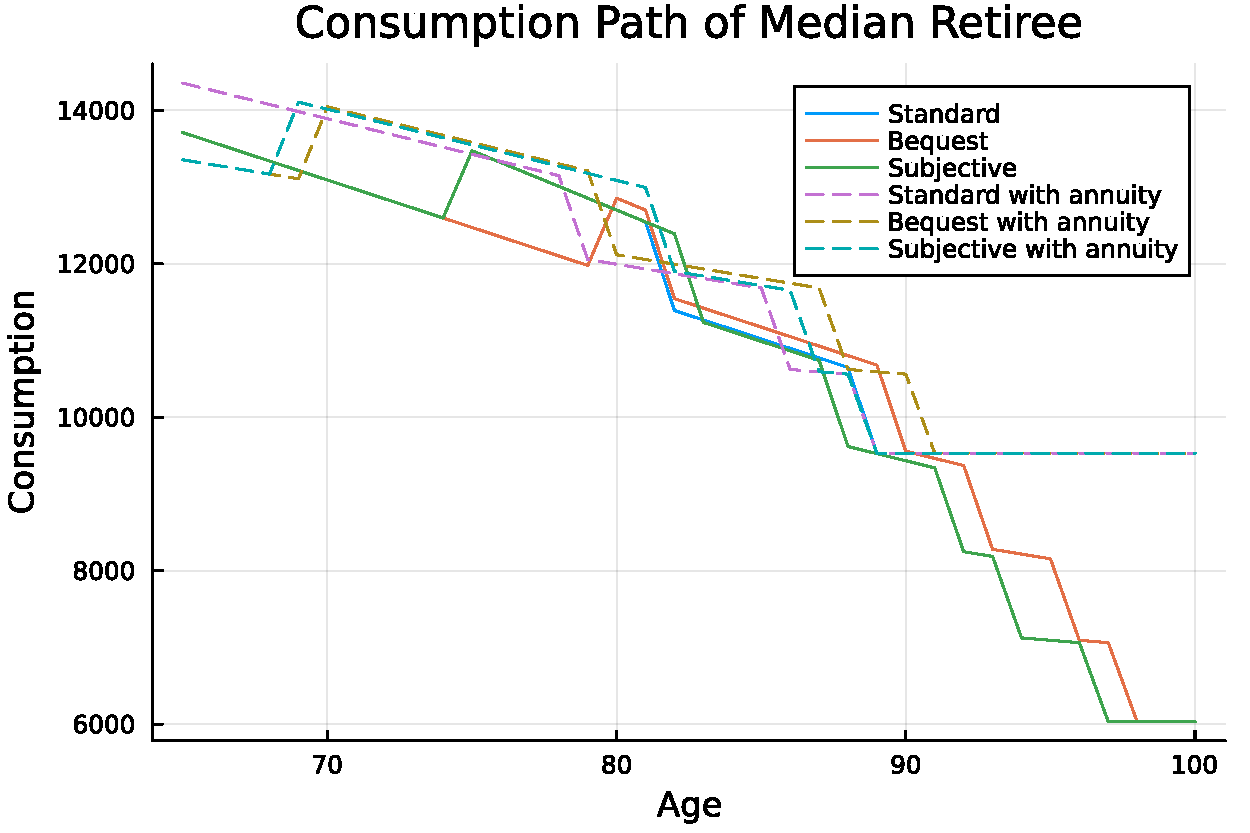
\includegraphics[width=0.7\columnwidth]{figures/consumption_plot_median_retiree.pdf}
    \label{fig:ConsumpPlot}
\end{figure}


\begin{figure}[h]
    \caption{Assets in retirement}
    \centering
    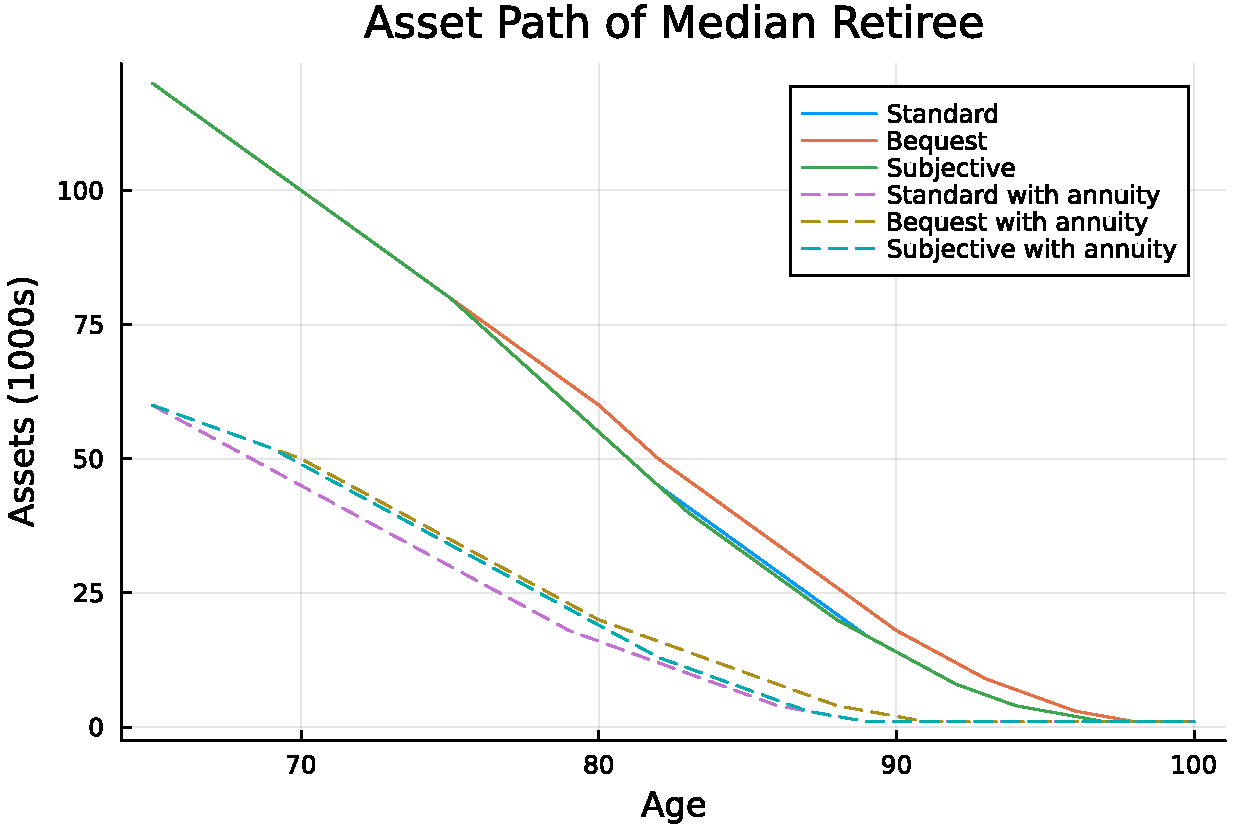
\includegraphics[width=0.7\columnwidth]{figures/asset_plot_median_retiree.pdf}
    \label{fig:AssetPlot}
\end{figure}

Figures \ref{fig:ConsumpPlot} and \ref{fig:AssetPlot} show the retirement path
of consumption and assets for a median retiree. This hypothetical woman has
£120,000 of assets at age 65 when they retired in 2012 with a state pension
income of £6000. The dashed lines show consumption and assets with an annuity
that costs half of their wealth. This buys them £3500 of annuity income, which,
given their objective life expectancy is a money's worth of about 90\%.

We can see that the asset path with the bequest motive keeps more for longer but
still decreases, and by their late 90s they have completely run down their
wealth. Interestingly, the asset path with the quickest run down is the standard
lifecycle model using objective life expectancies, which points towards this
individual being optimistic about their life chances. Also rather surprisingly
the asset paths of all three types are similar without annuities. The paths only
diverge after age 75 at which point the bequest path stays high and the other
paths start to decrease faster. This is contrary to the path with annuities
where the standard path diverges from the bequest and subjective paths
immediately.

The consumption paths all start at around £14,000 a year. The three models without an
annuity start at exactly the same amount and stay that way until the individual
reaches her mid seventies -- showing that even quite different lifecycle models
can generate similar paths. As expected, the consumption path with the bequest
motive with an annuity is lower at the start of retirement than the bequest path
without an annuity as individuals seek to build their savings back up. But it is
also lower for the subjective life expectancy case, again pointing toward this
individual being optimistic. However, the subjective consumption line rises at a
younger age than the line with bequests, showing that the models align with the
prediction that subjective lifecycle agents consume more in early retirement
compared to the other lifecycle models.

It is worth noting that the period of interest of this study is early retirement
and although differences across the lifecycle are not large, there are
significant differences at the start of retirement. This shows that different
lifecycle models will produce substantive differences in predictions, so knowing
which model is correct is important for policy.

I first round an ELSA individual's financial wealth to the nearest point on the
discrete asset grid, and do likewise for an individual's state pension income. I
then take the treatment group and evaluate their consumption in the year of
interview with an annuity, given that they annuitised 50\% of their financial
wealth in their retirement year. I also evaluate consumption without
annuitisation. The treatment group did not need to annuitise their wealth so I
use their predicted consumption from the lifecycle models with their starting
values of assets and pension income taken from their values in the ELSA dataset.
To be clear, the only individuals for whom I annuitise wealth are those with DC
pension pots who retired before 2014.

Because I discretised the state space, annuity prices are rounded down to the
nearest income grid point. I set the money's worth of annuities to $0.9$ when
calculating annuity prices but because I round down to the nearest income grid
point the real money's worth an individual receives is lower. I assume that
those who have a DC pension have half of their financial wealth in it since this
matches roughly what is seen in the summary statistics, so, for the untreated
group -- those who retired pre-reform -- I annuitise half of wealth. However,
since some individuals cannot buy a £500 annuity, which relates to one grid
point, with half of their financial wealth I only annuitise when an individual
has financial assets large enough to cross this threshold. I do not let these
individuals, with low assets, annuitise, setting consumption with and without an
annuity to the same amount.


\begin{table}

\caption{Model consumption predictions \label{tab:simulation_prediction}}
\centering
\begin{tabular}[t]{lrrrrrr}
\toprule
\multicolumn{1}{c}{ } & \multicolumn{2}{c}{Mean} & \multicolumn{2}{c}{Non Missing} & \multicolumn{2}{c}{Sd} \\
\cmidrule(l{3pt}r{3pt}){2-3} \cmidrule(l{3pt}r{3pt}){4-5} \cmidrule(l{3pt}r{3pt}){6-7}
 & Control & Treat & Control & Treat & Control & Treat\\
\midrule
Bequest & 891.3230 & 1041.2196 & 98 & 49 & 553.5802 & 540.8520\\
Standard & 918.5339 & 1068.4305 & 98 & 49 & 602.9341 & 573.0909\\
Subjective & 1018.3042 & 1144.9085 & 98 & 49 & 720.9637 & 597.3735\\
Total Monthly (ELSA) & 763.5413 & 887.8606 & 98 & 49 & 367.2683 & 538.9208\\
\bottomrule
\end{tabular}
\end{table}


Table \ref{tab:simulation_prediction} shows the mean of consumption that each
lifecycle model predicts for the treated and control groups as well as the
original mean of consumption from the ELSA data for the individuals with
non-missing values. The sample size of those with a DC pension is greatly
reduced. This is mainly because not everyone in the ELSA data answers the life
expectancy questions and of those who do answer some give answers that we cannot
use for reasons listed in the data section.

We can see the means for the control group are higher than the treated mean for
all models but there is significant difference between the original level of
consumption in the control group. The bequest and standard model both predict
lower consumption than the subjective model which is not surprising given the
subjective lifecycle individuals generally think their lives will be shorter and
therefore can consume more early in retirement. Likewise, it makes sense the
bequest model is lower than both other models since there is extra utility to be
gained from saving so that one can bequest to their heirs.

I now run the empirical models from above on this simulated data. This lets us
see which lifecycle model gives us the closest match to the coefficients seen in the
real data. We can therefore predict how other policy changes will impact
behaviour as well as predict the full path for assets and consumption later into
retirement. Matching a full model with method of simulated moments, though
possible using the entire ELSA data like \textbf{cite paper eric sent me}, does
not allow us to use incorporate policy changes into model.

\begin{landscape}
    \begin{table}

\caption{Simulated standard lifecycle models \label{tab:StandardLifeCycle}}
\centering
\begin{tabular}[t]{ldddd}
\toprule
  & {DCOnly} & {AllDataDCInteraction} & {DCOnlyPensionInt} & {DCOnyFinancialInt}\\
\midrule
(Intercept) & -681.172 & -648.121 & -681.816 & -588.159\\
PostReform & 2.841 & -4.678 & 0.558 & 30.651\\
RetiredAge & 10.688 & 10.332 & 10.714 & 9.088\\
FinWealth(£000s) & 4.433 & 4.316 & 4.435 & 4.512\\
Gender & 13.066 & 23.299 & 12.707 & 14.345\\
DCValue(£000s) & 0.000 & 0.001 & -0.006 & {}\\
YearsSinceRetirement & -6.223 & -0.621 & -6.492 & -7.268\\
OwnsHouse & 14.666 & 21.488 & 15.294 & 13.215\\
StatePension & 89.059 & 89.236 & 89.086 & 89.271\\
DCPension & {} & -15.382 & {} & {}\\
DBPension & {} & 1.522 & {} & {}\\
PostReform:DCPension & {} & 17.764 & {} & {}\\
PostReform:DBPension & {} & -11.353 & {} & {}\\
PostReform:DCValue(£000s) & {} & {} & 0.007 & {}\\
PostReform:FinWealth(£000s) & {} & {} & {} & -0.219\\
\midrule
Num.Obs. & 139 & 584 & 139 & 147\\
R2 & 0.995 & 0.993 & 0.995 & 0.995\\
R2 Adj. & 0.994 & 0.993 & 0.994 & 0.995\\
\bottomrule
\end{tabular}
\end{table}

\end{landscape}

\begin{landscape}
    \begin{table}

\caption{Simulated bequest lifecycle models \label{tab:BeqLifeCycle}}
\centering
\begin{tabular}[t]{lcccc}
\toprule
  & DCOnly & AllDataDCInteraction & DCOnlyPensionInt & DCOnyFinancialInt\\
\midrule
(Intercept) & \num{-447.672} & \num{-543.511} & \num{-448.371} & \num{-439.946}\\
PostReform & \num{16.687} & \num{-10.850} & \num{14.207} & \num{24.811}\\
RetiredAge & \num{7.577} & \num{9.155} & \num{7.605} & \num{7.446}\\
FinancialWealth (thousands) & \num{4.076} & \num{4.071} & \num{4.078} & \num{4.103}\\
Gender & \num{13.731} & \num{19.651} & \num{13.342} & \num{13.384}\\
DCValue (thousands) & \num{0.001} & \num{0.001} & \num{-0.005} & \\
YearsSinceRetirement & \num{-1.225} & \num{-0.888} & \num{-1.517} & \num{-2.273}\\
OwnsHouse & \num{5.064} & \num{17.853} & \num{5.746} & \num{3.839}\\
StatePension & \num{84.422} & \num{84.994} & \num{84.451} & \num{84.404}\\
DCPension &  & \num{-20.629} &  & \\
DBPension &  & \num{0.556} &  & \\
PostReform:DCPension &  & \num{25.529} &  & \\
PostReform:DBPension &  & \num{2.655} &  & \\
PostReform:DCValue (thousands) &  &  & \num{0.008} & \\
PostReform:FinancialWealth (thousands) &  &  &  & \num{-0.061}\\
\midrule
Num.Obs. & \num{139} & \num{584} & \num{139} & \num{147}\\
R2 & \num{0.996} & \num{0.995} & \num{0.996} & \num{0.996}\\
R2 Adj. & \num{0.995} & \num{0.995} & \num{0.995} & \num{0.995}\\
AIC & \num{1420.0} & \num{5938.7} & \num{1419.6} & \num{1496.3}\\
BIC & \num{1449.4} & \num{5999.9} & \num{1451.9} & \num{1526.2}\\
Log.Lik. & \num{-700.021} & \num{-2955.338} & \num{-698.814} & \num{-738.142}\\
RMSE & \num{37.23} & \num{38.15} & \num{36.91} & \num{36.69}\\
Std.Errors & HC3 & HC3 & HC3 & HC3\\
\bottomrule
\end{tabular}
\end{table}

\end{landscape}

\begin{landscape}
    \begin{table}

\caption{Simulated subjective lifecycle models \label{tab:SubjectiveLifeCycle}}
\centering
\begin{tabular}[t]{ldddd}
\toprule
  & {DCOnly} & {AllDataDCInteraction} & {DCOnlyPensionInt} & {DCOnyFinancialInt}\\
\midrule
(Intercept) & -1026.675 & -779.754 & -1025.583 & -1031.885\\
PostReform & -62.876 & -14.694 & -59.004 & 63.140\\
RetiredAge & 16.559 & 12.666 & 16.516 & 16.386\\
FinWealth(£000s) & 5.054 & 4.749 & 5.050 & 5.433\\
Gender & -62.495 & -30.426 & -61.888 & -52.366\\
DCValue(£000s) & 0.002 & 0.008 & 0.012 & {}\\
YearsSinceRetirement & -33.070 & 1.922 & -32.613 & -42.024\\
OwnsHouse & 66.452 & 44.938 & 65.386 & 51.098\\
StatePension & 92.846 & 92.993 & 92.800 & 91.539\\
DCPension & {} & 7.564 & {} & {}\\
DBPension & {} & -13.519 & {} & {}\\
PostReform:DCPension & {} & -30.893 & {} & {}\\
PostReform:DBPension & {} & 16.740 & {} & {}\\
PostReform:DCValue(£000s) & {} & {} & -0.012 & {}\\
PostReform:FinWealth(£000s) & {} & {} & {} & -0.949\\
\midrule
Num.Obs. & 139 & 584 & 139 & 147\\
R2 & 0.961 & 0.943 & 0.961 & 0.966\\
R2 Adj. & 0.958 & 0.942 & 0.958 & 0.964\\
\bottomrule
\end{tabular}
\end{table}

\end{landscape}


Tables \ref{tab:StandardLifeCycle}, \ref{tab:BeqLifeCycle} and
\ref{tab:SubjectiveLifeCycle} show the results. Each column in the table shows a
different empirical model that was applied to the data in the first part of this
paper. The first column just takes those with DC pensions, the second looks at
all individuals, whilst the third and fourth have interactions with financial
wealth and DC pension wealth.

Comparing the DC-only column across tables we can see that simulated bequest
model gives us the highest increase in consumption as a result of the reform.
This could be because this type of individual was previously saving out of the
annuity income to regain assets, so when they do not need to buy an annuity
anymore their consumption actually increases. Surprisingly, the predictions from
the lifecycle model using subjective life expectancies actually has a decreasing
coefficient on the reform even though on average for a given individual
consumption should increase as shown by the simple comparison in means. However,
this difference could be the result of the post-reform group having higher
subjective life expectancies, and therefore their consumption would be lower
than the control group.

The lifecycle model that is closest to the empirical models shown in Table
\ref{tab:DcOnlyRes} is the bequest model which gives an increase of 17 in
monthly consumption. However, this coefficient is just under half of the change
estimated in Table \ref{tab:DcOnlyRes} and reflects only a 0.6\% rise in
consumption after the reform.

In the second column, the coefficient of interest is the DC pension interaction
with the treatment variable since I use the difference in difference setup
again. The bequest model has a coefficient of 25.6, the standard model one of
17.7 and the standard model with subjective life expectancies has one of -30.9.
These coefficients are higher than the coefficient seen in Table
\ref{tab:ElsaAllData} with the predictions from the standard model matching the
coefficient in the empirical model best. The subjective model again has the
opposite sign to the one seen in the empirical model.

The interaction models in columns 3 and 4 both have correct signs for the main
reform effect in the standard and bequest models, although in both the
interaction with financial wealth has a negative coefficient showing that the
increase in consumption caused by the reform was progressively lower for those
who would have had to annuitise more wealth. In the subjective model table the
signs are again wrong apart from for the main treatment effect in the financial
interaction column. The lifecycle model that appears closest to the empirical
results is again the bequest model, which matches the signs from Tables
\ref{tab:DcOnlyInteract} and \ref{tab:DcOnlyFinWealthInteract}, but the
coefficients are smaller.

Across all regressions, the lifecycle model using subjective life expectancies
does not match the change in consumption that is seen when using ELSA data. It
is surprising that the consumption response is also very different to the other
lifecycle models used. One possible explanation for this could be that the
control and treatment groups have quite different sets of objective life
expectancies which therefore cause different consumption paths in early
retirement. The structure that the Weibull distribution imposes on the
transition probabilities could also be causing discontinuities in a given
individuals subjective probability of death between two periods, which would
impact how they consume across that part of retirement.

The evidence just presented points towards the bequest model being best able to
replicate the consumption response in the data. As highlighted above, the
benefit of having a theoretical model is that we can trace out future values of
consumption for individuals, only needing to know their starting point. So using
the bequest solution to the retirement problem, I plot the whole path of average
consumption and assets for the ELSA treated cohort. This plot is shown in the
figure below.



\textbf{Also get some plots of consumption in early retirement with and without
    annuities for the different model types}


\section{Conclusion}


\subsection{Rough plan}
\begin{itemize}
    \item Intro
          \begin{enumerate}
              \item "Latest data from HM Revenue Customs (published in April)
                    showed more than £45bn has been taken from pots since 2015."
                    https://www.ftadviser.com/pensions/2022/02/08/pension-freedoms-were-they-really-a-good-idea/
              \item what portion of savings are because of retirement savings?
              \item Also talk about heterogeneity across countries. Some
                    countries want to move towards more annuitisation. This
                    annual review is a good source of info
                    \cite{banks_crawford_ar_2022}
              \item https://www.moneysavingexpert.com/savings/pension-freedom/
          \end{enumerate}

          \textbf{Follow up by changing chat because the parameter estimates for
              the diff in diff have changed a bit -- DONE but check again when I
              have gone through it -- haven't checked the comparisons }


    \item \textbf{Abstract}
    \item \textbf{Talk about covariate balance table? We could just set it for
              the DC groups. }
    \item \textbf{Add bit about testing just those people who retired when they
              expected to retire.}
    \item \textbf{Could add consumption and retirement year plot?}
    \item \textbf{Maybe a small discussion of controls for the main regression
              tables as well}
    \item Conclusion
\end{itemize}



\bibliographystyle{chicago}
\bibliography{references}
\end{document}